
\chapter{On offshore wind farm maintenance scheduling for decision support on vessel fleet composition }
\label{Chap:ejor}
\ifpdf
\graphicspath{{X/figures/PNG/}{X/figures/PDF/}{X/figures/}}
\else
\graphicspath{{X/figures/EPS/}{X/figures/}}
\fi

The following chapter is an extension of Chapter \ref{Chap:iccs2017}.
%\begin{abstract}
%Maintenance costs account for a large part of the total cost of an offshore wind farm. Several models have been presented in the literature to optimize the fleet composition of the required vessels to support maintenance tasks. We provide a mixed integer linear programming (MILP) description of such a model, where on the higher level, the fleet composition is decided and on the lower level the maintenance operations are scheduled for a set of weather and breakdown scenarios. A drawback of deciding a perfect information schedule for the coming year is that in fact, the weather outcomes and breakdowns are not known in advance. Consequently, given a fleet composition, its corresponding maintenance costs are underestimated compared to what can be realised in practice under incomplete information. Therefore, we present several heuristics that simulate the practical scheduling and may provide a better cost estimate. The latter method is used to evaluate a fleet composition based on available information and it is compared with the MILP solution based on complete information.
%You did not make a greedy heuristic for fleet composition. Just a herustic scheduler for maintenance operations. You do not compare generated fleet, but you evaluate two fleet compositions. The outcomes of the procedure are compared to the underestimated fleet composition of the complete information MILP approach for a practical instance.
%\end{abstract}

%\begin{keyword}
%Scheduling \sep Offshore Wind Farm \sep Heuristic \sep Fleet composition \sep Maintenance planning
%\end{keyword}

%\end{frontmatter}


\section{Introduction}


The offshore wind energy industry is expected to continue its growth tendency in the near future. The European Wind Energy Association expects in its Central Scenario by 2030 a total installed capacity of 66 GW of offshore wind in the EU \cite{WES2030}.
%
Offshore wind farms (OWFs) are large scale infrastructures, requiring a large fleet of vessels able to perform operations and maintenance (O\&M) tasks on the installed turbines. The O\&M constitutes a large part of the costs of running an OWF installation, being up to one third of the OWF costs \cite{Snyder20091567}. Moreover, the fleet makes the installations  depend on non-renewable energy resources. Therefore, optimising the efficiency of the resources used for the O\&M tasks of an OWF becomes extremely important in order to make them economically viable and to reduce CO2 emissions.

Recent deterministic and stochastic model formulations for vessel composition and  optimization of maintenance operations at OWF's can be found in \cite{Gundegjerde2015} and \cite{HALVORSENWEARE2013}. A recent literature review on DSS for OWF's is given by \cite{hofmannrev}.
%
In~\cite{LijuanDai,EJOR2016} and \cite{STALHANE201592}, a model for maintenance routing and scheduling at offshore wind farms based on the Dantzig-Wolfe decomposition method has been implemented.
In that work, a mixed integer linear program is solved for each subset of turbines to generate all  feasible routes and maintenance schedules for the vessels for each period.
The routes take several constraints into account, such as weather conditions, the availability of vessels and the number of technicians available at the operation and maintenance base.
%
In~\cite{Stalhane2016357}, a two-stage stochastic programming model is presented to determine a cost-optimal fleet size and mix for O\&M tasks at offshore wind farms for the total expected lifetime of the OWF. For that, the study considers time periods fixed to three months.

The basis of our investigation is a scenario based MILP model which like the models in \cite{HALVORSENWEARE2013} and \cite{Stalhane2016357} decides on the vessel fleet composition. All these models evaluate the value of the vessel fleet composition and base selection based on scheduling with perfect information; the weather conditions and breakdowns happening during a scenario of a year are known beforehand. The research question in the current paper is whether the vessel fleet composition may be affected when maintenance scheduling is done in a heuristic way following a practical decision rule given the available information at the time of maintenance scheduling.

We investigate this question in the following way. Section \ref{sec:problemdescriptionEJOR} describes the practical decision problem of operating an OWF and selecting a fleet to support its maintenance tasks. Section \ref{sec:mathematicalformulation} describes an MILP model, which simultaneously determines the maintenance scheduling as well as the fleet composition. In Section \ref{sec:heuristic}, a heuristic for the operational stage of the model is presented. Section \ref{sec:computationalstudyEJOR} presents a computational study used to compare the outcomes of both procedures. Finally, Section \ref{sec:conclusion} summarises our findings.


\section{Problem definition}
\label{sec:problemdescriptionEJOR}

This section describes the maintenance planning problem related to a fleet of vessels for an offshore wind farm during a planning horizon, based on a more extensive model of fleet size and mix decisions in~\cite{Elin}. The aim is to find an optimal fleet of vessels and a collection of maintenance tasks to be performed on the wind turbines. That model contains a detailed description of the operational scheduling dealing with each individual action. Our vision also distinguishes  periods (shifts) of 12 hours, but aggregates a number of tasks in each period (shift).


\emph{Preventive} as \emph{corrective} maintenance tasks are considered.
Preventive maintenance tasks are meant to prevent failures and prolong the lifetime of wind turbines. Examples include visual inspection, changing of consumables, oil sampling, and tightening of bolts \cite{obdam}. Corrective maintenance tasks are needed to repair broken down wind turbines. There is a one-to-one correspondence between failure types and corrective task types.


The number of necessary preventive tasks of each type to be performed is predefined at the beginning of the year. Corrective tasks are only needed after a specific failure occurs in a wind turbine. The planner is confronted in each scenario with failures occurring dynamically. There is a downtime cost associated to the lack of electricity production in turbines during the execution of a maintenance task. Downtime costs are also considered for broken down turbines, incurred for the shifts from diagnose until reparation.




To perform the maintenance tasks, a fleet of vessels is needed. Vessel types have properties such as the type of maintenance tasks they can perform, capacity for transferring technicians, a depreciation cost over the planning horizon, a sailing speed and a threshold for wind speed and wave height that prevents to transfer technicians to the turbines or sailing if they are exceeded. Every vessel is associated to a base, from which it travels to the wind farm to perform maintenance tasks. Each base has a certain vessel capacity, a capacity to accommodate technicians, an associated cost and coordinates which provide its distance to the wind farm.

The decision problem includes a number of candidate bases that can be used and a number of vessel types associated to them. Each vessel type is able to support a particular set of patterns, from the base they are associated with. A pattern consists of one or several maintenance tasks to be performed at the OWF that fits in a shift, including the time it takes the vessel type to perform a round trip visiting the OWF from their base. For each shift the available vessels are able to perform a single pattern of the possible ones that are associated to their type and their base. Some patterns from different vessel types and associated to different bases might be virtually the same, containing the same list of tasks to be performed during the shift. Their cost and time required may vary, considering the speed of the vessel or the distance from their base to the OWF.  Some task types do not require the vessel to be present at the turbine. This facilitates performing several tasks in parallel in a single time shift. It is irrelevant whether  a pattern contains tasks that run in parallel or sequentially, as long as they meet the time constraints of a shift and the vessel type can accommodate enough technicians to perform the tasks. Moreover, some task types take longer than the time available in a single shift. These long tasks are split into smaller parts that fit with the duration of the shifts. If a long task is initiated in one shift, it does not necessarily have to be continued in the following. However, for corrective tasks, downtime costs are incurred for all shifts until the task is finished and the failure in the turbine has been repaired.

Decisions actually take place on two levels: the first (tactical) level decides which bases to use and which vessels should be available during the planning horizon period under consideration. The second (operational) level schedules operations  including which patterns to support by which available vessel in every shift of the planning horizon. The random events the planner is confronted with consist of weather conditions preventing use of vessels for maintenance and the possible failures of turbines that require corrective maintenance tasks.



\section{MILP model description}
\label{sec:mathematicalformulation}

Like in the models of \cite{HALVORSENWEARE2013} and \cite{Stalhane2016357},
%Elin says this are not the papers....
 the tactical level decisions are evaluated based on a scenario approach, where the planner has perfect information to schedule the operational maintenance tasks. The following symbols are used to describe the mathematical optimisation model.


%\scalebox{1}{
\begin{tabular}{ll}
	\multicolumn{2}{l}{Sets}\\
	%K
	%V
	$\mathcal{K}$ 				& 	Set of bases \\
	$\mathcal{V}_k$ 				& 	Set of vessel types at base $k$ \\
	$\mathcal{S}$ 				& 	Set of scenarios \\	
%	$\mathcal{T}$ 				& 	Set of time periods in the planning horizon \\	
	$\mathcal{T}_{vs}$			&	Set of shifts not suitable for sailing due to weather limitations \\
								&	for vessel type $v$ during scenario $s$\\
	$\Gamma$ 					&	Set of maintenance task types \\
	$\mathcal{NP}$				&	Subset of planned preventive maintenance task types, $\mathcal{NP}\subset\Gamma$ \\
	$\mathcal{NC}$				&	Subset of corrective maintenance task types, $\mathcal{NC}\subset\Gamma$ \\
	$\mathcal{P}$				&	Set of all possible patterns\\
	$\mathcal{P}_{kv}$			&	\parbox[t]{10cm}{Set of possible patterns for a vessel of type $v$ operating from base $k$}\\
\end{tabular}



\begin{tabular}{ll}
	\\
  \multicolumn{2}{l}{Parameters}\\
	$T$ & Number of shifts in the planning horizon\\
	$F_{k}$ 	&	Fixed cost per year of operating base $k$\\
	$G_{v}$ 	&	\parbox[t]{10cm}{Charter or depreciation cost for using a vessel of type $v$ over the complete planning horizon}\\
	$D_{st}$	&	\parbox[t]{10cm}{Income loss due to downtime of performing a maintenance task in scenario $s$ in shift $t$} \\
	$H_{ts}$ 		&	\parbox[t]{10cm}{Hourly income loss due to downtime of performing a maintenance task in scenario $s$ in shift $t$}\\
	%This is actually D_st / 12, being 12 in this case the number of hours of a shift
	$C_{p}$ 	&	\parbox[t]{10cm}{Cost of executing pattern $p\in \mathcal{P}_{kv}$ from base $k$ and a vessel of type $v$ }\\
	$CP_i$ 	&	\parbox[t]{10cm}{Penalty cost for not executing a preventive maintenance task of type $i\in \mathcal{NP}$}\\
%	\end{tabular}
	
%\begin{tabular}{ll}
	%\\
  \multicolumn{2}{l}{}\\	
	%$NI_{i}$ 		&	Number of hours required by preventive maintenance task $i$\\
	$N_{i}$ 		&	\parbox[t]{10cm}{Number of hours required to execute maintenance task of type $i\in \Gamma$ during the planning horizon}\\
	$PP_{i}$ 		&	\parbox[t]{10cm}{Number of planned preventive maintenance tasks of type $i\in \mathcal{NP}$}\\	
	$M_{k}$ 		&	\parbox[t]{10cm}{Number of maintenance technicians available at base $k\in K$ in each shift}\\
	$MP_{p}$ 		&	\parbox[t]{10cm}{Required number of maintenance technician personnel to execute pattern $p$} \\
	$Q_{kv}$ 	&	\parbox[t]{10cm}{Maximum number of vessels of type $v$ that can operate from base $k$}\\
	$B_{i}$ &	\parbox[t]{10cm}{Hours spent on a task of type $i$ in one shift, being $B_i \leq N_i$}\\
	$A_{ip}$ 		&	\parbox[t]{10cm}{Number of tasks of type $i$ in pattern $p$}\\
	$P_s$ 		&	Probability of scenario $s$\\
	$Y_{its}$ 	& 	\parbox[t]{10cm}{Number of failures of type $i\in\mathcal{NC}$ accumulated in shifts $1,\ldots,t$ in scenario $s$}.
	\\
%\end{tabular}
%}

%\begin{tabular}{ll}
	\\
	\multicolumn{2}{l}{Tactical decision variables}\\
	$y_{k} \in \{0,1\}$ 	& Equal to 1 if base $k$ is used, 0 otherwise\\
	$x_{kv} \in\{0,\ldots,Q_{kv}\}$ &	Number of vessels of type $v$ operated from base $k$\\
	\\
	%
%\end{tabular}	

%\begin{tabular}{ll}	
	\multicolumn{2}{l}{Operational decision variables}\\
	$w_{its}\in\mathbb{Z}^+$	&	\parbox[t]{9.5cm}{Number of corrective maintenance tasks of type  $i \in\mathcal{NC}$ supported during shift $t$ in scenario $s$}\\
	$q_{its} \in\mathbb{Z}^+$	&	\parbox[t]{9.5cm}{Number of preventive maintenance tasks of type $i \in \mathcal{NP}$ supported during shift $t$ in scenario $s$}\\
	$u_{pts}\in\mathbb{Z}^+$ &	\parbox[t]{9.5cm}{Number of vessels executing pattern $p$ during shift $t$ in scenario $s$}\\
	$\bar{w}_{its}\in\mathbb{Z}^+$	&	\parbox[t]{9.5cm}{Number of corrective maintenance tasks of type  $i \in\mathcal{NC}$ that are not (yet) completed in scenario $s$ in shift $t$}\\
	$\bar{q}_{i s}\in\mathbb{Z}^+$	&	\parbox[t]{9.5cm}{Number of preventive maintenance tasks of type $i \in \mathcal{NP}$ not completed in scenario $s$ at the end of the planning horizon}  \\
								\\	
\end{tabular}

In order to solve the model, the bounds on the variables should be set as sharp as possible to facilitate pre-solving operations of an LP solver that filters out those variables that have a value of zero and those constraints that are not binding. We define the following bounds:


\begin{align}
\label{eq:bound1}
  0 \leq x_{kv} \leq Q_{kv},				&\quad	\forall k,v\\
\label{eq:bound2}
  0 \leq u_{pts} \leq \sum\limits_{k\in\mathcal{K}} \sum\limits_{v\in\mathcal{V}_k} Q_{kv} &\quad \forall p,s,t  \\
\label{eq:bound3}
0 \leq w_{its} \leq \sum\limits_{k\in\mathcal{K}} \sum\limits_{v\in\mathcal{V}_k} Q_{kv}\max\limits_{p\in \mathcal{P}_{kv}}A_{ip} 	&\quad \forall i \in \mathcal{NP}, \forall t,s\\
\label{eq:bound4}  	
0 \leq q_{its} \leq \sum\limits_{k\in\mathcal{K}} \sum\limits_{v\in\mathcal{V}_k} Q_{kv}\max\limits_{p\in \mathcal{P}_{kv}}A_{ip} 	&\quad \forall i \in \mathcal{NC}, \forall t,s\\
\label{eq:bound5}
  0 \leq \bar{w}_{its}\leq Y_{i ts} &\quad	\forall i\in\mathcal{NC}, \forall t,s\\
\label{eq:bound6}
   0 \leq \bar{q}{is}\leq PP_{i} &\quad	\forall i\in\mathcal{NP}, \forall s
\end{align}



The value of parameter $Q_{kv}$ is an upper bound on the number of vessels that can be used from each base. Therefore, the number of patterns that can be performed in a shift for a particular scenario is bounded by the total capacity of vessels for the considered bases. The number of corrective tasks not finished at a certain shift is bounded above by the total occurrences of failures $Y_{its}$ thus far.
The number of preventive tasks not performed at the end of the horizon is bounded by the total number of planned preventive tasks $PP_i$.


\subsection{Objective function}

The objective is to minimise the fixed costs of operating the bases and the charter cost of the selected vessels, the costs of all performed patterns throughout the planning horizon, the downtime costs associated with the running maintenance tasks or persistent failures and the penalty costs of preventive and corrective task types that are not finished within the planning horizon:
%
\begin{align}
\label{eq:objfun}
 \min  	\sum\limits_{k\in \mathcal{K}} F_k y_k  %1
	      + \sum\limits_{k\in \mathcal{K}}\sum\limits_{v\in\mathcal{V}_k} G_v x_{kv} %2
	      + \sum\limits_{s\in\mathcal{S}} P_{s} \left(\sum\limits_{k\in\mathcal{K}} \sum\limits_{v\in\mathcal{V}_k} \sum\limits_{p\in\mathcal{P}_{kv}} \sum\limits_{t=1}^T C_{p}u_{pts}\right) +\\ \nonumber
	     \sum\limits_{s\in\mathcal{S}} P_{s} \left(\sum\limits_{i\in \mathcal{NP}}  \sum\limits_{t=1}^TH_{ts}B_{i}q_{its}
+ \sum\limits_{i \in\mathcal{NC}} \sum\limits_{t=1}^T D_{st} \bar{w}_{its} +  \sum\limits_{i \in\mathcal{NP}} CP_i \bar{q}_{is} + \sum\limits_{i \in\mathcal{NC}} CP_i \bar{w}_{iTs}\right)
\end{align}
%
The first two terms of the objective function (\ref{eq:objfun}) cover the costs for the tactical decisions: cost of bases and vessels. The first term refers to the fixed costs for operating the chosen base(s) during the  planning horizon. The second defines the charter costs for the available fleet of vessels during the  planning horizon.

The following terms cover the expected operational costs of the model. Therefore, the cost of each scenario is  multiplied by its probability. The third term of the objective function (\ref{eq:objfun}) determines the cost of operating the patterns during the planning horizon. Terms four and five describe the downtime costs of preventive and corrective task types, respectively. While the downtime costs for preventive task types are only incurred while a task is taking place on a turbine, downtime for corrective task types initiate from the moment the breakdown occurs and continues until the shift in which it has been repaired. The last two terms are related to penalty costs. Term six is the penalty incurred for the preventive maintenance task types that are not performed within the planning horizon while term seven is the penalty for not finishing all corrective tasks.



\subsection{Constraints for tactical decisions}

There is only one constraint on the tactical level describing the usual relation that base $k$ should be in use, if one wants to station vessels there, and set the bounds of the maximum number of each vessel type for each base.

\begin{align}
\label{eq:const1:maxVkfromK}
  x_{kv} \leq Q_{kv}y_{k}  	&	&	\forall k, v
\end{align}
%
 The tactical decision directly influences the possibilities of the operational planning. A larger fleet allows to perform more patterns each shift.

\subsection{Constraints on operational decisions}
Constraints on the operational level are given by the following inequalities:
\begin{align}
\label{eq:const1}
  %\sum\limits_{\{p|k_p=k,v_p=v\}} u_{pts}\le x_{kv}, 			&\quad		\forall k,v,t,s\\
  \sum\limits_{p\in \mathcal{P}_{kv}} u_{pts}\le x_{kv}, 			&\quad		\forall k,v,t,s\\
  \label{eq:const4}
  %\sum\limits_{\{p|k_p=k\}} MP_{p}u_{pts} \leq M_{k},				&\quad	\forall k,s,t\\
  \sum\limits_{v\in V_k}\sum\limits_{p\in \mathcal{P}_{kv}} MP_{p}u_{pts} \leq M_{k},				&\quad	\forall k,s,t\\
  \label{eq:const5}
   \sum\limits_{p\in \mathcal{P}_{kv}} A_{ip}u_{pts} - q_{its}\geq 0,				&\quad	\forall i\in \mathcal{NP}, \forall k,v,s, t\\
   \label{eq:const6}
   \sum\limits_{p\in \mathcal{P}_{kv}} A_{ip}u_{pts} - w_{its}\geq 0,				&\quad	\forall i\in \mathcal{NC}, \forall k,v,s, t\\
\label{eq:const:rw}
  \frac{N_{i}}{B_{i}}(Y_{its}-\bar{w}_{its}) \leq  \sum\limits_{\tau=1}^t  w_{i\tau s}\leq \ceil{\frac{N_{i}}{B_{i}} Y_{its}}, 		 &\quad	\forall i \in\mathcal{NC}, \forall s,t\\
    %\frac{N_{i}}{B_{i}}(Y_{its}-\bar{w}_{its}) \leq  \sum\limits_{\tau=1}^t \sum\limits_{p \in \mathcal{P}} w_{i\tau s}\leq \ceil{\frac{N_{i}}{B_{i}} Y_{its}}, 		 &\quad	\forall i \in\mathcal{NC}, \forall s,t\\
\label{eq:const3}
   N_{i}\bar{q}_{is}+ \sum\limits_{t=1}^T B_{i}q_{its}\ge N_{i}PP_{i}, 		&\quad \forall i \in \mathcal{NP}, \forall s\\
\label{eq:constweather}
   	u_{pts}=0, &\quad \forall p\in \mathcal{P}, \forall t \in \mathcal{T}_{vs}, \forall s
\end{align}
%
Constraint \eqref{eq:const1} bounds operations on the availability of sufficient vessels at each base. Each available vessel has the potential to contribute performing one of its possible patterns each shift.
Constraint \eqref{eq:const4} limits operations due to available personnel at the bases.
Constraints \eqref{eq:const5} and \eqref{eq:const6} link the assignment of individual tasks to planned patterns and availability of vessels, for preventive and corrective types respectively. It is necessary to keep track of not finished corrective tasks every shift, as the turbines affected incur downtime costs until they are fixed.
The lower bound of constraint \eqref{eq:const:rw} keeps track of the number of not finished corrective tasks (breakdowns). The planner cannot complete more corrective tasks than the ones present at the OWF every shift. The upper bound ensures that the number of single type tasks does not exceed the number of broken down turbines caused by the same failure type. Also, a single corrective task of type $i$  contributes with $B_i$ hours during a shift, while $N_i\geq B_i$ hours are needed to complete the a complete task of type $i$. Therefore, the number $\frac{N_i}{B_i}Y_{its}$ should be rounded up allowing the last part of a large task to be performed. Otherwise, in case just one corrective task of type $i$ is needed and $B_i\nmid N_i$, the task could not be finished until another failure of type $i$ occurs, increasing$Y_{its}$. For preventive tasks it is only necessary to check the number of not performed tasks at the end of the time horizon. Constraint \eqref{eq:const3} keeps track of the number of preventive tasks for each type that have not been finalised in scenario $s$.

Implicitly, constraints \eqref{eq:const:rw} and \eqref{eq:const3} imply that the individual task schedule follows from a FIFO approach for preventive and corrective task types, where the first task that has been started is the first to be ended. Such assumption is needed: if each task was treated as an independent task the model would become intractable for small instances. Finally, constraint \ref{eq:constweather} prevents patterns to be performed during shifts in which the weather conditions exceed the threshold of wind speed or wave height for the vessel type used to execute the pattern.



%Constraints \eqref{eq:constsomany} and \eqref{eq:only1fori} guarantee that in one shift at most one operation is contributing to each task.
\subsection{Generating columns (bundles and patterns) for the model}
\label{subsec:buildpatterns}
%\subsection{Generation of bundles and patterns}
The basic decisions of the scheduler of the maintenance operations are based on feasible patterns, previously crafted by the decision maker. This section describes an automatic procedure to generate the feasible maintenance patterns for every base and vessel type combination. A recursive algorithm can be used for this task, considering constraints such as the number of technicians needed or the time limitations to complete the pattern.

As sketched in Section \ref{sec:problemdescriptionEJOR}, some task types do not require the vessel to be present at the turbine during the operation such that these types can be run in parallel. We will indicate them by the set $\Gamma p_v$. Therefore, the generation of columns is based on a two-step procedure. First, we generate the feasible set of bundles of tasks that include only task types from $\Gamma p_v$ that can be run in parallel using a recursive procedure described in Algorithm \ref{alg:buildbundle}. In the second step, we combine these bundles with the non-parallel task types in $\Gamma n_v$ to create the final set of patterns.


A bundle $b$ is specified as a quadruple (List, Time, Cost, Tech) specifying the list of activites, the time to execute it, the cost and the number of technicians required, respectively. Each task in List is performed at a different turbine and they are run in parallel. During the execution of a bundle, the vessel docks to the first turbine, offloads the task materials and technicians required and then moves to another turbine until all the tasks are started. When finished, the vessel recollects the technicians and returns to base. The duration (Time) of a bundle consists of the set up time (setupTime$_i$) for its tasks and the docking time (docktime$_v$) at each turbine when dropping off and when picking up the technicians. With respect to the time $B_i$ spent on a single task, we have to keep in mind they are run in parallel. The procedure has to take into account the number of technicians Tech$_v$ allowed on vessel $v$ and the number of hours TMX$_v$ it may stay at the Offshore wind farm. Finally, the cost of a task Cost$_i$ and the number of required technicians Tech$_i$ is updated.

%Elin said to put the alg. after explaining all the parameters etc...

\begin{algorithm}[h]
	\caption{build\_bundle(Bundle $b$, Vessel $v$)}
	\label{alg:buildbundle}
	\begin{algorithmic}
		%\REQUIRE say here
		%\ENSURE say here
		\medskip
		\FOR {all $i\in \Gamma p_v$}
		\STATE $T_{vi}$= 2*dockTime$_v$+setupTime$_i$;
		%\IF {$v$ not needed in turbine for task $i$\green{This if is not needed after declaring $\Gamma p_v$. Parallel task and not needed in turbine ar equivalent}}
		\STATE temp\_time=max(Time+$T_{vi}$,$B_i$+$T_{vi}$)
		\STATE temp\_cost= Cost+Cost$_i$
		\STATE temp\_tech= Tech + Tech$_i$
		\STATE temp\_list by adding $i$ to List
		\IF {temp\_time $\leq$ TMX$_v$ and temp\_tech $\leq$ Tech$_v$}
		\STATE define new bundle $\hat b$=(temp\_list,temp\_time,temp\_cost,temp\_tech)
		\STATE $\mathcal{B}_v= \mathcal{B}_v\cup \{\hat b\}$
		\STATE build\_bundle($\hat b$,$v$)
		%\ENDIF
		%\ENDIF
		\ENDIF
		\ENDFOR	
	\end{algorithmic}
\end{algorithm}
The procedure, starting with $b=(\emptyset, 0, 0, 0)$ builds a set $\mathcal{B}_v$ of bundles of tasks for each vessel using the set of tasks $\Gamma$ specified for each vessel $\Gamma_v$. The lists of the bundles are unordered with repetitions of the same task types.
To create a sharp set description, a dominance procedure is run over the bundle sets. Let List$_1$ and List$_2$ be such that List$_1 \subseteq$ List$_2$, then the bundle with List$_1$ is removed.

\begin{algorithm}[h]
	\caption{Generate Patterns}
	\label{alg:generatepatterns}
	\begin{algorithmic}
		%\REQUIRE say here
		%\ENSURE say here
		\medskip
		\FOR {all $k\in \mathcal{K}$ and $v\in \mathcal{V}_k$}
			\STATE determine Time from 2*(distance to OWF)/(vessel speed of $v$);
			\STATE determine Cost from 2*(distance to OWF)*(CostFuel per km of $v$);
			\STATE $p$=pattern($\emptyset$, Time, Cost, 0)
			\FOR {tasks/bundles  $n$ in $\Gamma n_v$ and $\mathcal{B}_v$}
				\STATE build\_pattern($p$,$n$)
			\ENDFOR
		\ENDFOR
		\STATE\RETURN $\mathcal{P}_{kv}$
		%\EndProcedure
		%\vskip 5pt
	\end{algorithmic}
\end{algorithm}

After Algorithm \ref{alg:buildbundle} is run for every vessel type and the dominance procedure is performed to each vessel type bundle set, they can be used to build the final pattern set.
\begin{algorithm}[h]
	\caption{build\_pattern(Pattern $p$, Activity $n$)}
	\label{alg:buildpattern}
	\begin{algorithmic}
		\medskip
		%this has not been used! \STATE $N_b$= Number of bundles for vessel $v$ and base $k$
		%\IF {$n<|\Gamma|$}
		%\STATE $T_a=v$.ActTime($n$)
		\IF {$n \in \Gamma n_v$ (vessel needed at turbine)}
		\STATE temp\_time=Time+2*dockTime$_v$+setupTime$_n$+actTime$_n$
		%\STATE temp\_cost= $p$.Cost+2 C\_transit + C\_act($n$)
		\STATE temp\_cost= Cost+ cost$_n$
		\STATE temp\_tech= Tech + Tech$_n$
		\STATE temp\_list= List $\cup \{n\}$
		\IF {temp\_time $\leq v$.TMX}
		\STATE new pattern $\pi$ := (temp\_list, temp\_time,temp\_cost,temp\_tech)
		\STATE $\mathcal{P}_{kv}= \mathcal{P}_{kv}\cup \pi$
		\STATE build\_pattern($\pi$,$n+1$)
		%\ENDIF
		\ENDIF
		\ELSE
		% implicitly, n is a bundle \IF {$n\leq |\Gamma|+|B_v|$}
		\STATE temp\_time= Time+Time$_n$, i.e. $n$ is a bundle
		\STATE temp\_cost= Cost+Cost$_n$
		\STATE temp\_tech= Tech+Tech$_n$
		\STATE temp\_list= List $\cup$ List$_n$
		\IF {temp\_time $\leq v$.TMX}
		\STATE $w$=(temp\_list, temp\_time, temp\_cost, temp\_tech)
		\STATE $\mathcal{P}_{kv}= \mathcal{P}_{kv}\cup \{w\}$
		\STATE build\_pattern($w$,$n+1$)
		%\ENDIF
		\ENDIF
		\ENDIF
		%\STATE\RETURN $q$
		%\EndProcedure
		%\vskip 5pt
	\end{algorithmic}
\end{algorithm}
Algorithms \ref{alg:generatepatterns} and \ref{alg:buildpattern} use the dominated bundle sets $\mathcal B_v$ and the non-parallel task types to derive the pattern sets $\mathcal P_{kv}$. Since the time to arrive to the OWF depends on the cruising speed of the vessel types and the distance from the departure base to the OWF, pattern sets are associated with a base and a vessel type. Algorithm \ref{alg:generatepatterns} goes over each base and vessel type combination starting by adding the time of a return trip to the OWF and the fuel costs as a base for the time and the costs of the patterns of each vessel type and base combination. Then, patterns are build recursively in Algorithm \ref{alg:buildpattern}, which is called from Algorithm \ref{alg:generatepatterns} $|B_v|$ times (existing bundles) and $|\Gamma n_v|$ times, i.e. the number of non-parallel task types.





\section{Operational scheduling based on available information}
\label{sec:heuristic}
In this Section, we discuss a heuristic (a scheduler) for the operational stage of the model, where a plan should be generated for every shift of a particular scenario, depending on the weather constraints. In contrast to the MILP approach, no  anticipation of the weather conditions and the failures in the turbines is taken. With respect to the available information, the parameters of the stochastic failure events are assumed not to be known. For the weather realisations, only the monthly averages of wind speed are known, based on historic weather data. At the beginning of each shift, the weather conditions for it and the new failures are realised.

The scheduler consists of two parts. First, the part called OWFscheduler harvests and deals with the available information. The second part (heuristic) evaluates the possible patterns to be performed for every shift, deciding which of the available vessels to use and which patterns to perform.
%
At the beginning of each shift, the OWFscheduler administrates the occurring failures and the weather circumstances for the current shift. This is fed to the heuristic with the decisions for the current shift. The scheduler administrates the incurred costs for the performed pattens and the number of hours invested in each task type at the OWF.
\begin{algorithm}[h]
	\caption{OWFscheduler}
	\label{alg:scheduler}
	\begin{algorithmic}
		%\REQUIRE say here
		%\ENSURE say here
		\medskip
		\FOR { $i\in \mathcal{NP}$}
			\STATE RemainHours$_i=PP_i\times N_i$
			%\STATE RemainAct$_i=PP_i$
		\ENDFOR
		\FOR {$t\in \{1,\ldots,2T\}$}
			\STATE Observe realised  wind$_t$ and wave$_t$; $\mathcal{VP}_t=\emptyset$
			\FOR {$v$ with a $k$ for which $x_{kv}>0$}
				\STATE $\mathcal{VP}_t=\mathcal{VP}_t \cup \{v\}$ if wind$_t<$maxWind$_v$ AND wave$_t<$ maxWave$_v$
				\STATE Add observed failure type $i$ to DownAct$_i$
				%\STATE For i in $\mathcal{NC}$: tDownAct(i)=tDownAct(i)+fail\_period(p,i)
				\STATE Update downtime costs
			\ENDFOR
			\STATE Call Heuristic
			\ENDFOR
		\STATE Calculate total cost
		%\EndProcedure
		\vskip 5pt
	\end{algorithmic}
\end{algorithm}
\subsection{The scheduler}
The scheduler starts by taking the realisation of the weather circumstances, including wind speed, wind$_t$, and wave height, wave$_t$, for the current shift $t$.
%I deleted this, it can only confuse the reviewer...
%Shifts are considered 12 hours long, but weather resolution is generally shorter, only a few hours long. The scheduler maps the chosen shift $t$ with their corresponding values for wind speed and the values for wave height. The weather data used in this study has a resolution of six hours. So, for our study, the algorithm fetches two data both for wind speed and wave height per shift.


From these values, the vessels that cannot sail during shift $t$ are discarded via the data maxWind$_v$ and maxWave$_v$ for the maximum wind speed and wave height supported by each vessel type. Let $\mathcal{VP}_t$ represents the list of vessels that execute perform patterns during shift $t$. The scheduler puts observed new failures occurring at shift $t$ on a stack. The downtime costs due to corrective failures is administrated considering the number of failures at the OWF after the operations have taken place, matching with the MILP formulation in Section \ref{sec:mathematicalformulation}.

\begin{algorithm}[h]
	\caption{Heuristic}
	\label{alg:heuristic}
	\begin{algorithmic}
		%\REQUIRE say here
		%\ENSURE say here
		\medskip

		%\WHILE {goIDLE=0}	
			\STATE Set $\mathcal{P}_t$ of possible patterns
			given $(t,\mathcal{VP}_t$,  DownAct$_i$,RemainHours$_i$)\label{alg:line:allpatcosts}
			\STATE Determine fitness $f_p$ for each pattern $p \in\mathcal{P}_t$
			\STATE Find $r=\arg\min_{p\in \mathcal{P}_t} f_p$
			\STATE Determine IdleCost
			\WHILE{patterns possible and IdleCost$<f_r$}				
				\FOR{ Choosen pattern $r$ and tasks $i\in$ List$_r$}
				\STATE Update downtime costs for $i \in \mathcal{NP}$;
				\STATE RemainHours$_i = $RemainHours$_i -B_i*A_{ir}$
				\STATE Update DownAct$_i$ for $i\in \mathcal{NC}$
				\STATE Remove the used vessel and update $\mathcal{P}_t$ correspondingly
				\STATE Update $f_p, p\in \mathcal{P}_t$, idleCost and $r$
				\ENDFOR
			\ENDWHILE
		%\ENDWHILE

		\vskip 5pt
	\end{algorithmic}
\end{algorithm}
%Describing Allpatcosts
The scheduler calls the heuristic which chooses the patterns to be performed (associated to one of the available vessels operating from its base) and updates the remaining time of the tasks with respect to shift $t$. The scheduler continues after the heuristic finishes executing, moving to the next shift or, at the end of the time horizon, calculating and returning the final cost for the operational stage.



\subsection{The heuristic}
\label{subsec:heuristic}
The heuristic chooses the patterns to be performed during the current shift $t$, $\mathcal{P}_t\subset \mathcal{P}$. It considers the available vessels $\mathcal{VP}_t$, the state of the needed tasks RemainHours$_i$ (which resembles the number of needed hours to finish all of the tasks of type $i$) and the realisation of the weather data for the current shift $t$,in order to evaluate the downtime costs. The set $\mathcal{P}_t$ is fed from the existing patterns for the vessels that, after realising the weather conditions, are able to sail, $\mathcal{VP}_t$. For that, procedure patternfitness, gives a fitness value $f_p$ for each of the possible patterns to be performed during the shift.%, and returns a list containing all the options with fitness called allpat.

The heuristic selects the pattern with the minimum fitness value $f_p$ and compares it with the cost value of not performing more patterns during the current shift, captured in parameter idleCost. This parameter reflects the downtime cost for the turbines that are down due to a failure, the only cost that applies during a particular period in case no patterns are performed. If a minimum fitness pattern is selected, the heuristic updates the corresponding downtime cost for preventive tasks and the number of remaining hours for every task type, RemainHours$_i$, are reduced. %It is important to update the state of the problem after every pattern has been chosen, as performing a patter, potentially reducing failures, may affect further decisions. The vessel corresponding to the pattern allpat($r$) is
Moreover, the vessel used by pattern $r$ is removed from $\mathcal{VP}_t$ and the set of possible patterns is updated, removing from $\mathcal{P}_t$ the remaining patterns associated with the chosen vessel. This process continues until there are no available pattern in $\mathcal{P}_t$. In practice this means that all of the available vessels have been chosen to either perform one of their patterns or staying at their bases.% . The heuristic follows repeating this process until either the current pattern costs for allpat($r$) is higher than idleCost or the set of available vessels $\mathcal{VP}_t$ is empty. %(checked by allpat $=\emptyset$).

\subsection{Procedure patternfitness}
For a greedy like heuristic that iteratively selects the most promising pattern, the evaluation of the fitness $f_p$ based on the available (updated) information is essential. In our case, the following information can be weighted.

\begin{itemize}
	\item Pattern cost: the cost of performing pattern $p$
	\item Downtime costs for turbines that are shut down to perform the tasks included in pattern $p$
	\item Potentially saved penalty costs $SPC_p$ obtained by performing pattern $p$% potentially saved, $S_{PC}$ (Potential Saved Penalty Costs, change name...)
	\item Saved downtime costs \emph{Scosts}$_p$ of performing pattern $p$ % (downtime costs for fixed failures during $p$)
\end{itemize}
%
The sum of this costs give the fitness $f_p$ of pattern $p$.
Including pattern costs and downtime costs for shut down turbines is straightforward. The calculation of $S{PC}$ and \emph{Scosts} is detailed in the next paragraphs. Unlike the first two terms, $SPC$ and \emph{Scosts} are negative.
%\begin{figure}
%	\centering
%	\includegraphics[scale=0.6]{}
%	\caption{}
%	\label{}
%\end{figure}
\begin{figure}[hbt]
	\begin{center}
		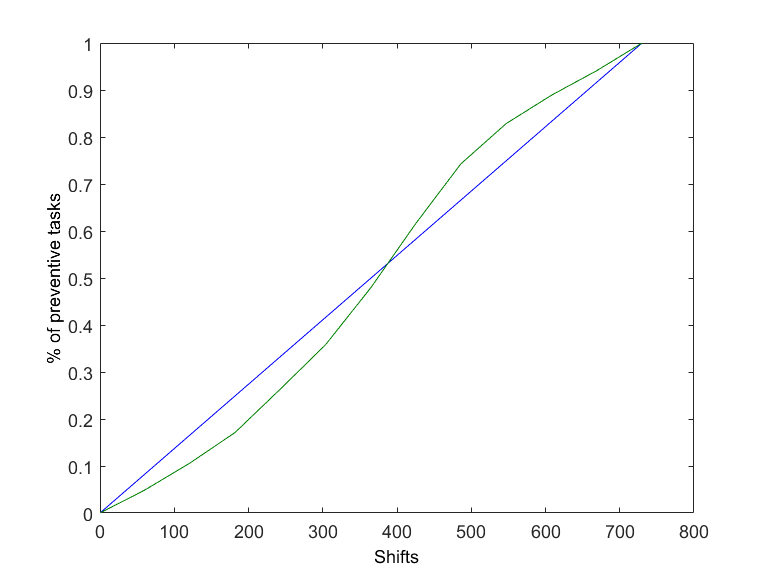
\includegraphics[scale=0.5]{EJOR/figures/developactivities.png}
	\end{center}
	\caption{Linear and monthly average approaches to guide scheduling preventive tasks}
	\label{fig:monthavg}
\end{figure}
$SPC_p$ refers to the proportion of the penalty costs based on the time pattern $p$ spends on its different tasks types. If, for instance, one of the tasks of $p$ constitutes $\beta$\% of the total time of a particular task type, the $\beta$\% of the penalty cost of that task type is counted. However, the penalty for not performing preventive tasks during the year is rather high and patterns consisting on those tasks could be overly chosen. One way to proceed could be to limit the number of  preventive tasks that can be scheduled linearly with time.  In that case, the number of preventive tasks of type $i$ that can be finished up by shift $t$ would be $ \frac{PP_it}{2T}$. However, gains can be obtained by scheduling more tasks when, seasonally, wind speed is expected to be slower. Performing preventive tasks when the wind speed is low saves downtime costs due to performing preventive tasks, as reflected by parameter $D_{st}$.
In practice, the weather conditions are not known to the planner beforehand, but the scheduler has insight in the monthly average conditions for wind speed, based on historic data. From these averages it can be derived the expected power loss for a single turbine during month $\tau$, which we assume to be captured by the average values $w_\tau$. One can normalise these values to obtain the proportion of expected loss of month $\tau$ respect to the total year: $\bar{w}_\tau=\frac{w_i}{\sum_{j=1}^{12}w_i}$. One would like to perform in month $\tau$ a fraction of the total planned preventive tasks that is inversely proportional to the number $\bar{w}_\tau$. This fraction is given by $\varphi_{\tau}=\frac{1}{\bar{w}_\tau}\frac{1}{\sum_{j=1}^{12}\bar{w}_j}$, dividing again by the total summation of $\bar{w}_j$ to normalise results.
%
Figure \ref{fig:monthavg} depicts the accumulative values of $\varphi_{t}$ interpolated between the month averages confronted with a linear approach.
%
Consequently, parameter BehindSch is determined for each $i\in \mathcal{NP}$ according to
$$BehindSch_{i}=\max((1-\varphi_{t})PP_i -\lceil \frac{RemainHours_i}{N_i}\rceil,0)$$
%
For corrective task types $i\in \mathcal{NC}$, we focus on the unfinished work
%
$$BehindSch_{i}= DownAct_i$$
%
Finally, to have a valuation $S{PC}_p$ for the pattern, we can add penalties $p_i$ leading to
%
$$SPC_p= \frac{t}{2T}\sum_{i \in \Gamma}p_iA_{ip}\frac{B_i}{N_i}Behindsch_i ,$$
%
Notice, this factor has a higher weight in the fitness when approaching the end of the horizon. However, if $Behindsch_i=0$ the valuation of $S{PC}_p$ is set to zero. If $Behindsch_i=0$ and for patterns that include one or more preventive type tasks, the wind speed is checked. In case it is lower than the expected average, the fitness valuation of $p$ is different: the pattern costs are not considered for the fitness and the number of hours of type $i$ that that pattern performs is calculated and subtracted from the fitness value.


The term \emph{scosts} is a negative value that refers to the potential savings in electricity production if a break down turbine is repaired. After calculating the contribution of pattern $p\in\mathcal{P}_{kv}$ for each  corrective task type $i\in \mathcal{NC}$ in terms of number of tasks performed, \emph{scosts} accumulates the value:
%
$$scosts=-nact(i)(2T-t)ydown$$
%
The term $ydown$ represents the average downtime cost of a single turbine for the total duration of the planning horizon. Notice, this factor gets a higher weight at the beginning of the planning horizon that than at the end.

% On Matlab, run script Untitled (I know...) to generate the data and the again.



%\subsection{Case $Behindsch_i=0$}
%\label{subsec:fitnessexception}
%For shifts in which preventive types are performed according to schedule, SPC does not count with the potentially saved costs for those types. $Behindsch_i=0$, the wind speed  is checked. In case is lower than the expected average, which is known, the pattern costs are not considered for the fitness. The number of hours of type $i$ that that pattern performs is calculated and subtracted from the fitness value.





%{algorithm}[h]
%	\caption{vesselcansail(Vessel $v$,shift $t$)}
%	\label{alg:vesselcansail}
%	\begin{algorithmic}
		%\REQUIRE say here
		%\ENSURE say here
%		\medskip
		%\FOR { $i\in \{1,\ldots,12/6\}$ (Change 12 and 6 for parameters)}
		%\STATE $n=12/6 (t-1)+i$
%		\RETURN {wind($n$)$<$maxWind($v$) AND wave($n$)$<$ maxWave($v$)}
		%\RETURN false;
		%\STATE EXIT;
		%\ENDIF
		
		%\ENDFOR
		%\RETURN true;
		%\STATE\RETURN return something?
		%\EndProcedure
		%\vskip 5pt
%	\end{algorithmic}
%\end{algorithm}


\section{Computational illustration}
\label{sec:computationalstudyEJOR}

In the MILP model, the lower level operational planning cost provides a lower bound for the incurred cost due to failures and downtime. By formulating the operational tasks in a one-shot model, in principle all the scenario is known beforehand and earlier tasks can be planned based on knowledge of failures that will occur later, i.e. anticipation is allowed. This makes the planning in principle cheaper than what is possible in reality. On the other hand, due to the  nature of the variable $\bar{w}_{its}$, there is a tension in the optimal outcome to start repairing a failure as soon as possible by a corrective task.

In this section, we discuss the amount of underestimation for specific realistic data confronting the optimal MILP outcome of the lower level for scenarios with the heuristic decision rule defined in Section \ref{sec:heuristic}.
%
The model and the heuristic have been compared for an instance similar to the one published in \cite{GutierrezAlcoba:ICCS2017}.

The MILP has been modelled for the bi-level model using GAMS interface \cite{gams}, and solved using the CPLEX solver, setting the optimality gap at 1\%.

\subsection{A case study}

We consider an OWF consisting of 125 turbines. The planning horizon is one year and the periods represent 12 hour shifts and include a return trip from the base the vessel is located to the OWF and a bundle of activities. In practical terms there are 730 periods. There are three available bases $B_1,B_2,B_3$ around the OWF, each of which can accommodate up to 48 technicians and they are located at 110, 61  and 86 kilometers respectively from the OWF. The cost of using each of them, for the entire time horizon is 2, 6 and 7 million monetary units (mu) respectively.

Four types of vessels are considered: $V_1,V_2,V_3,V_4$. Each base has space to allow two vessels of type $V_1$, two of type $V_2$, four of type $V_3$ and one of type $V_4$. Vessel type $V_4$ is able to accommodate up to 30 technicians, while the rest has space for only 12. The cost of having a vessel during the whole planning horizon for vessel types $V_1$, $V_2$, $V_3$ and $V_4$ is, respectively, 122,4000, 2,500,000, 750,000 and 7,200,000 mu. Vessel types $V_1$ and $V_2$ can travel at a speed of 20 knots, while vessel types $V_3$ and $V_4$ can travel at 40 knots. In practical terms this means that vessel types $V_1$ and $V_2$ require about 5.94, 3.3 and 4.64 hours to perform a return trip between bases $B_1$, $B_2$ and $B_3$ respectively while vessel types $V_3$ and $V_4$ would require half of that time, allowing more time to perform activities in each shift.

There are two preventive activity types $A_1,A_2$ and two corrective activity types $A_3, A_4$. All vessel types are able to perform all the activity types considered. Activity type $A_4$ requires the vessel supporting the operation to be present at the turbine while the activity is performed, whereas activity types $A_1,A_2,A_3$ can be run in parallel. The vessel drops a group of technicians at each turbine that is going to be supported during the shift. The time required to perform activity types $A_1$, $A_2$, $A_3$ and $A_4$ is 60 , 100 , 3 and 7.5 hours respectively. The maximum time per period and turbine that a group of technicians can support an activity type is 6 hours. Consequently, only activities of type $A_3$ can be performed in a single period. The penalty cost for not executing a preventive activity type is 10 million mu. For corrective activities of type $A_3$, the cost is 50,000 mu, and for type $A_4$, the penalty cost rises to 500,000 mu. The patterns for each combination of base and vessel type are generated following the procedure described in Algorithms \ref{alg:buildbundle} and \ref{alg:buildpattern}.

For our case study, there are 125 planned activities of type $A_1$ and 60 of type $A_2$. The number of corrective activity types corresponds to the number of failures of the turbines and depends on the scenario. A scenario consists of the events of the failures of the turbines and the weather conditions for every period. Failures that require corrective activity types $A_3$ and $A_4$ follow a binomial distribution. The rate of failures for a corrective activity of type $A_3$ is 5 times per turbine per year, and 3 times per turbine a year for failures that require an activity of type $A_4$. Weather conditions are taken from historical weather data. For each scenario, a report file containing a year of wind speed and wave height data of the OWF area is picked for feeding these variables.

\subsection{Discussion of results}

For comparing the performance of the heuristic for the operational stage with the optimal solution of the MILP problem, two different tactical stage decisions have been considered. The first one is  the optimal solution for the MILP, (S1), which consists of using three vessels of type $V_3$ from base $B_1$. An instance consisting on a tactical stage decision using less vessels than the optimal MILP solution based on perfect information, would not generate significant results. The second instance (S2) consists of using four vessels of type $V_3$ from base $B_1$.

A set of 20 scenarios have been generated. For each scenario, the heuristic has been run and the MILP problem has been solved for the tactical stage decisions studied, (S1) and (S2) the optimal solution for the MILP; using three vessels of type $V_3$ from base $B_1$ and (S2). Table \ref{tab:experiments} presents the average value of the 20 scenarios for the total cost, executing patterns cost, preventive and corrective downtime costs and operational stage costs for tactical stage decisions S1 and S2, running the heuristic and solving the MILP problem. Preventive and corrective penalty costs are not included in Table \ref{tab:experiments}, since they result to be zero for the generated scenarios.

\begin{table}[h]
	\centering
	\caption{Associated costs for the MILP optimal solution and the heuristic for tactical decisions S1 and S2}
	\label{tab:experiments}
\begin{tabular}{rrrrrr}
         & Total    & Pattern & P. D.   & C. D.   & Op. S. Cost \\
MILP S1  & 10986350 & 5060220 & 1117923 & 558265  & 6736408     \\
MILP S2  & 11472400 & 5126880 & 1028245 & 314890  & 6470015     \\
HEUR. S1 & 13401952 & 5346330 & 2296092 & 1509528 & 9151951     \\
HEUR. S2 & 12958671 & 5435595 & 1235124 & 1287951 & 7958671
\end{tabular}
\end{table}

The MILP complete information solution for S1 has a total cost of nearly 11 million monetary units (MU), while the heuristic for S1 has a cost of 13.4 million MU. Considering only the costs of the operational stage, the MILP complete information solution is 6.73 million MU, while the heuristic reaches 9.15 million MU. %For a few scenarios, the heuristic cannot finish all the preventive tasks, giving an average value for preventive penalty costs of 160000 MU.
Downtime costs for corrective tasks is about 2.7 times higher than the MILP cost. For preventive tasks the cost doubles that of the MILP solutions. This shows that the heuristic does not perform well for S1 with the optimal MILP perfect information setting. In a real setting, when failures and weather conditions are uncertain, that tactical decision might not be optimal.

However, for S2 the deviation between the two solutions is quite different. The MILP complete information solution for the operational stage is 6.47 million MU, reducing only slightly the costs of S1. However, the heuristic reduces that cost to 7.95 million MU, and this reduction comes mostly by handling preventive tasks much better, reducing the cost by half compared to the tactical decision S1. It can be observed that the downtime cost for corrective tasks, incurred by broken down turbines until they are repaired, is the only cost significantly higher for the heuristic compared to the MILP solution costs, for both tactical decisions S1 and S2. This can be explained considering that the MILP model has exact information for when the failures occur for all the periods of the problem, being able to anticipate corrective tasks early in time. In contrast, the cost of performing the patterns, which constitutes the major cost of operating the OWF and is not related with uncertain events, is only  6\% above the one provided by the MILP.





\section{Conclusion}
\label{sec:conclusion}
Models in the literature on selecting an optimal vessel fleet composition for operations and maintenance tasks at OWFs during a planning horizon typically apply a complete information approach to evaluate the fleet composition. The models are confronted with weather conditions and turbine failures. Weather conditions may prevent vessels sailing and execute tasks at the OWF, while turbine failures result in new corrective maintenance tasks. However, weather conditions and failures are unknown in practice. Therefore, a deterministic complete information approach to find the optimal solution for the operational stage only provides a lower bound on the maintenance costs in the operational stage. In the current paper, a similar MILP model for the fleet composition is presented. The question is: What are the costs if the scheduler applies a heuristic rule based on the information available in practice? This means, the heuristic is not based on perfect information, realising the weather and failure events at the beginning of each shift. The results show that the heuristic performs well  when the tactical decisions include enough vessels to cover the demand of O\&M activities at the OWF and allows for slack in the scheduling compared to the optimal complete information plan. Although the performance costs of the heuristic for the chosen scheduling are only 6\% above the optimal lower bound, for the corrective tasks, where (stochastic) failures have to be repaired, the cost is about four times higher than that given by the MILP. This illustrates the effect of anticipation in a perfect information situation. The value of evaluating the fleet composition in a realistic setting is that probably the chosen vessel plan will contain more vessels, as this facilitates recourse actions on random events.

%\bibliographystyle{plain}
%\bibliography{Tesis_Alejandro}


%\end{document}
